\subsection{Numerical Solvers}
\subsubsection{Implicit vs Explicit Solvers}
Numerical solvers are used to integrate the system dynamics over time, approximating the continuous evolution of a state $\dot{x} = f(t, x)$ through discrete time steps $\Delta t$. Depending on how the derivative is evaluated, integration schemes are categorized as either \textit{``explicit''} or \textit{``implicit''}.  
\\ \\
In an \textit{``explicit''} method, the state update is computed directly from known quantities at the current time step as such
$$
    x_{k+1} = x_k + \Delta t \, f(t_k, x_k)
$$
Making it simple and computationally efficient. However, explicit methods are only \textit{``conditionally stable''}, meaning the chosen time step must be sufficiently small to maintain numerical stability. In contrast, an \textit{``implicit''} method evaluates the derivative at the next time step,
$$
    x_{k+1} = x_k + \Delta t \, f(t_{k+1}, x_{k+1})
$$
This requires solving a nonlinear equation for $x_{k+1}$, often using iterative techniques such as the Newton-Raphson method. Implicit solvers are generally \textit{``unconditionally stable''}, allowing larger time steps and better handling of stiff systems, but at the cost of significantly higher computational complexity.  
\\ \\
Figure \ref{fig:system-modeling-stability-region-explicit-solvers} illustrates the stability regions of several explicit Runge-Kutta (ERK) methods of increasing order. As the order increases (eks ERK1 to ERK4), the stability region expands, allowing larger integration time steps before instability occurs. However, this improvement comes with additional intermediate evaluations of $f(t, x)$ per time step, increasing computational cost. Advanced explicit techniques, such as Adaptive Runge-Kutta methods (eks ARK4(5) or Dormand-Prince), further optimize stability by dynamically adjusting the time step, whereas implicit formulations like Gauss-Legendre Runge-Kutta (GLRK) offer superior stability at the expense of computational simplicity.  
\begin{figure}[H]
    \centering
    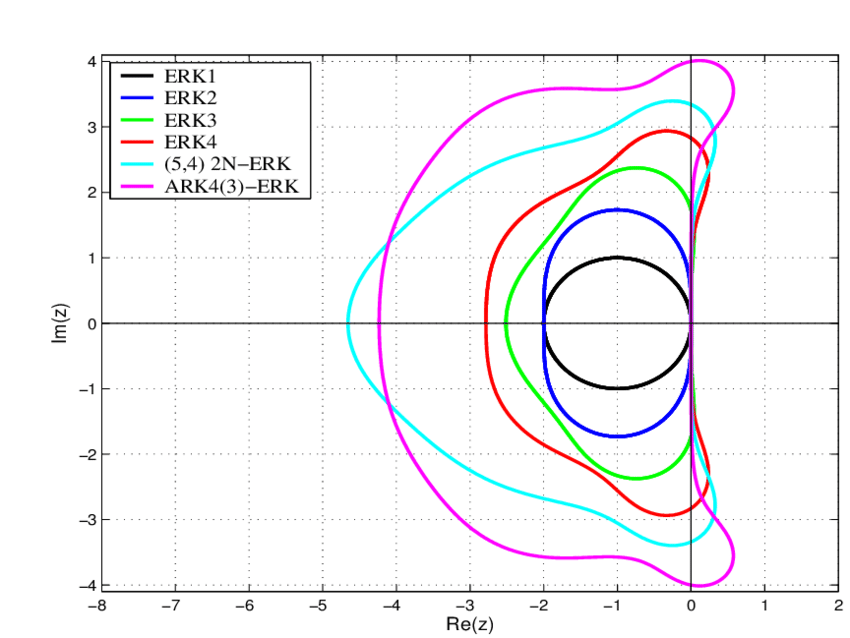
\includegraphics[width=0.9\linewidth]{Pictures/System_Modeling/Numerical_Solvers/StabilityRegionExplicitSolvers.png}
    \caption{Stability regions of various explicit Runge-Kutta methods. Higher order methods support larger integration time steps before instability occurs, at the cost of increased computational effort. Image taken from research paper on explicit and implicit numerical solvers.\textsuperscript{\cite{stability_region_explicit_solvers}}}
    \label{fig:system-modeling-stability-region-explicit-solvers}
\end{figure}
\noindent
In real-time navigation and estimation applications, such as the INS model implemented in this work, explicit solvers provide the optimal balance between accuracy and efficiency. Although implicit solvers are preferred for offline simulation or highly stiff systems, their iterative nature and computational load make them impractical for embedded execution. Moreover, any minor numerical drift introduced by the explicit integration scheme is compensated during sensor fusion, where aiding measurements (eks GNSS) correct accumulated errors at each update step.  
\\ \\
Overall, ERK methods, particularly the 4th order ERK4 formulation, offer an efficient and sufficiently accurate approach for forward state propagation in real-time marine navigation systems.



\subsubsection{Newton-Euler Method}
The Newton-Euler method represents the simplest and most direct approach to numerically integrating a systems dynamics over time. It forms the foundation for explicit state propagation in real-time navigation and control systems, providing a fast and straightforward way to approximate the continuous evolution of the system state.  
\\ \\
The general continuous time system is described by
$$
    \dot{\mathbf{x}} = f(\mathbf{x}, \mathbf{u})
$$
where $\mathbf{x}$ denotes the state vector, $\mathbf{u}$ represents the system inputs, and $f(\mathbf{x}, \mathbf{u})$ defines the continuous time motion model.  
\\ \\
Using the explicit or forward Euler discretization, the system is approximated over discrete time intervals $\Delta t$ as
$$
    \mathbf{x}_{k+1} = \mathbf{x}_k + \Delta t\,f(\mathbf{x}_k, \mathbf{u}_k)
$$
This update relies only on the current state and input, making the method fully explicit with no need for iteration or matrix inversion. Its direct formulation ensures minimal computational overhead, which is particularly important for real-time embedded execution.  
\\ \\
The Newton-Euler method is explicit, first order accurate, and computationally efficient. Its simplicity makes it ideal for systems where high update rates and frequent measurement corrections are available. However, it is conditionally stable, and numerical errors can accumulate for large time steps or rapidly changing dynamics. In aided estimation systems, these effects are typically compensated by sensor fusion corrections such as GNSS or magnetometer updates.  
\\ \\
Although higher order explicit methods like Runge-Kutta improve numerical accuracy, they require additional evaluations of $f(\mathbf{x}, \mathbf{u})$ and therefore increase computational cost. For real-time navigation and control, the Newton-Euler method provides an optimal trade-off between computational efficiency and integration accuracy, making it well suited for embedded state propagation in this work.
in this work.



\subsubsection{Runge-Kutta Methods (RK4)}
The Runge-Kutta family of methods generalizes the explicit Newton-Euler integration scheme by combining several intermediate evaluations of the system dynamics to achieve higher accuracy. The general continuous time system is written as
$$
    \dot{\mathbf{x}} = f(\mathbf{x}, \mathbf{u})
$$
where $\mathbf{x}$ represents the state vector and $\mathbf{u}$ the control inputs.  
\\ \\
The Runge-Kutta approach evaluates $f(\mathbf{x}, \mathbf{u})$ at multiple points within each time step $\Delta t$, and combines these intermediate slopes using a set of weighting coefficients defined by the Runge-Kutta formulation. This structure can be compactly represented using the Butcher tableau:
\\ \\
\begin{center}
    \begin{tabular}{c|cccc}
        $c_1$ &  \\
        $c_2$ & $a_{21}$ \\
        $c_3$ & $a_{31}$ & $a_{32}$ \\
        $c_4$ & $a_{41}$ & $a_{42}$ & $a_{43}$ \\ \hline
        & $b_1$ & $b_2$ & $b_3$ & $b_4$
    \end{tabular}
\end{center}
Each constant defines how intermediate stages are calculated and combined.  
\\ \\
For the classical 4th order Explicit Runge-Kutta (ERK4) method, the coefficients are given by:
\\ \\
\begin{center}
    \begin{tabular}{c|cccc}
        0 &  \\
        $\tfrac{1}{2}$ & $\tfrac{1}{2}$ \\
        $\tfrac{1}{2}$ & 0 & $\tfrac{1}{2}$ \\
        1 & 0 & 0 & 1 \\ \hline
        & $\tfrac{1}{6}$ & $\tfrac{1}{3}$ & $\tfrac{1}{3}$ & $\tfrac{1}{6}$
    \end{tabular}
\end{center}
Using these coefficients, the RK4 method is computed as
$$
\begin{aligned}
    k_1 &= f(\mathbf{x}_k, \mathbf{u}_k) \\
    k_2 &= f(\mathbf{x}_k + \tfrac{\Delta t}{2}k_1, \mathbf{u}_k) \\
    k_3 &= f(\mathbf{x}_k + \tfrac{\Delta t}{2}k_2, \mathbf{u}_k) \\
    k_4 &= f(\mathbf{x}_k + \Delta t\,k_3, \mathbf{u}_k) \\
    \mathbf{x}_{k+1} &= \mathbf{x}_k + \Delta t \sum_{i=1}^{4} b_i k_i
\end{aligned}
$$
Each $k_i$ represents an intermediate slope that estimates the systems rate of change at different points inside the time step. The final update is a weighted average of these slopes, providing a more accurate approximation of the state evolution compared to the single slope Newton-Euler approach.  
\\ \\
The RK4 method achieves a global truncation error of $\mathcal{O}(\Delta t^4)$, making it more accurate for smooth nonlinear systems. However, this improvement requires four evaluations of $f(\mathbf{x}, \mathbf{u})$ per integration step, which increases computational cost and memory usage.  
\\ \\
The Newton-Euler method can be viewed as the 1st order Explicit Runge-Kutta scheme (ERK1), where only a single evaluation of $f(\mathbf{x}, \mathbf{u})$ is used. While ERK4 provides higher numerical precision, its added complexity offers minimal benefit in real-time embedded systems where aiding sensors, such as GNSS or magnetometers, continuously correct small integration errors.  
\\ \\
In practical navigation and estimation systems, especially on embedded platforms, the Newton-Euler (ERK1) method remains the preferred choice due to its low computational load and sufficient accuracy. ERK4 is mainly reserved for offline simulation or analysis, where increased precision justifies the additional computational effort.


